\documentclass[12pt]{report}

\usepackage{amsmath,amssymb,amsfonts} %In case we need math stuff
\usepackage{graphicx} %For inserting images and stuff
\usepackage{listings} %For inserting code snippets
\usepackage{enumerate} %For fancy enumeration
\usepackage{hyperref}
\usepackage{pdfpages}
\usepackage{float}
\usepackage[margin=2cm]{geometry} %Nice margin setting

\title{ECSE 321 - Intro to Software Engineering\\Design Specification Document - Deliverable 2}
\author{Harley Wiltzer\\Camilo Garcia La Rotta\\Jake Shnaidman\\Robert Attard\\Matthew Lesko}
\date{February 27, 2017}

\begin{document}
\pagenumbering{gobble} %No page number on title page
\maketitle
\newpage
\pagenumbering{arabic} %Arabic numeral page numbers on regular pages
\tableofcontents
\part{Architecture of the Proposed Solution}
\section{Description}
	The software architecture comprises of two different patterns: a Model/View/Controller pattern
	and a Layered Architecture pattern. An "Authentication and Authorization" layer is on top of the
	MVC layer. Once the user is authenticated and authorized, they have access to the MVC layer. The
	MVC system contains three components which interact with each other: 
	\begin{itemize}
		\item Controller
		\item View
		\item Model
	\end{itemize}
	The Model component manages the system data and associated operations on that data; it
	encapsulates all the entities that are part of the model (can be seen in the model class
	diagram). The View component defines and manages how the data is presented to the user. The
	Controller component manages user interaction (key presses, mouse clicks, etc.) and passes these
	interactions to the View and the Model.
\section{Rationale}
	The MVC pattern was chosen because this allows the components to be changed independently. For
	example, adding a new view or changing an existing view can be done without any changes to the
	underlying data in the model. It allows the data to change independently of its representation
	and vice versa. Moreover, it supports presentation of the same data in different ways with changes made in
	one representation shown in all of them. \\
	Furthermore, the Model-View-Controller pattern makes multiplatform development very convenient.
	Using this paradigm, equivalent code may be generated for the model component on all platforms,
	as the model is isolated from the other components. Then, the views are isolated from the
	controllers so that modifications to the view classes do not affect code for other platforms
	that utilize the controller classes.\\
	The Layered Architecture pattern was used because the user would need to first authenticate
	him/herself and then receive authorization in order to interact with the sublayer.
\section{Block Diagram}
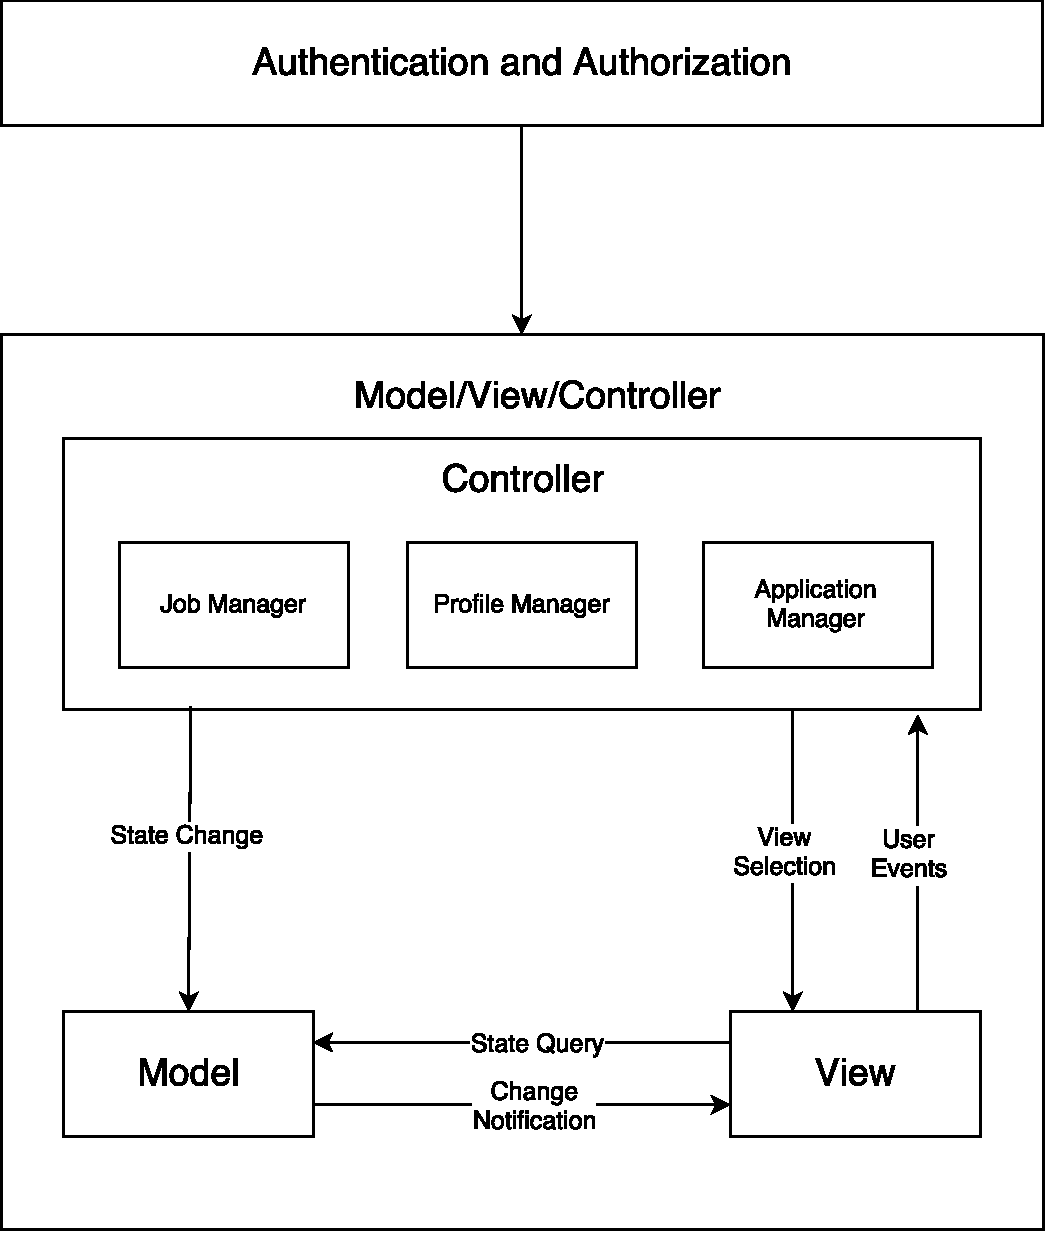
\includepdf[scale=0.5,pages=1]{Architecture/blockDiagram}

\part{Description of the Detailed Design}
The Domain Model changed significantly since the last Deliverable, and the new domain model may be
found below.\\
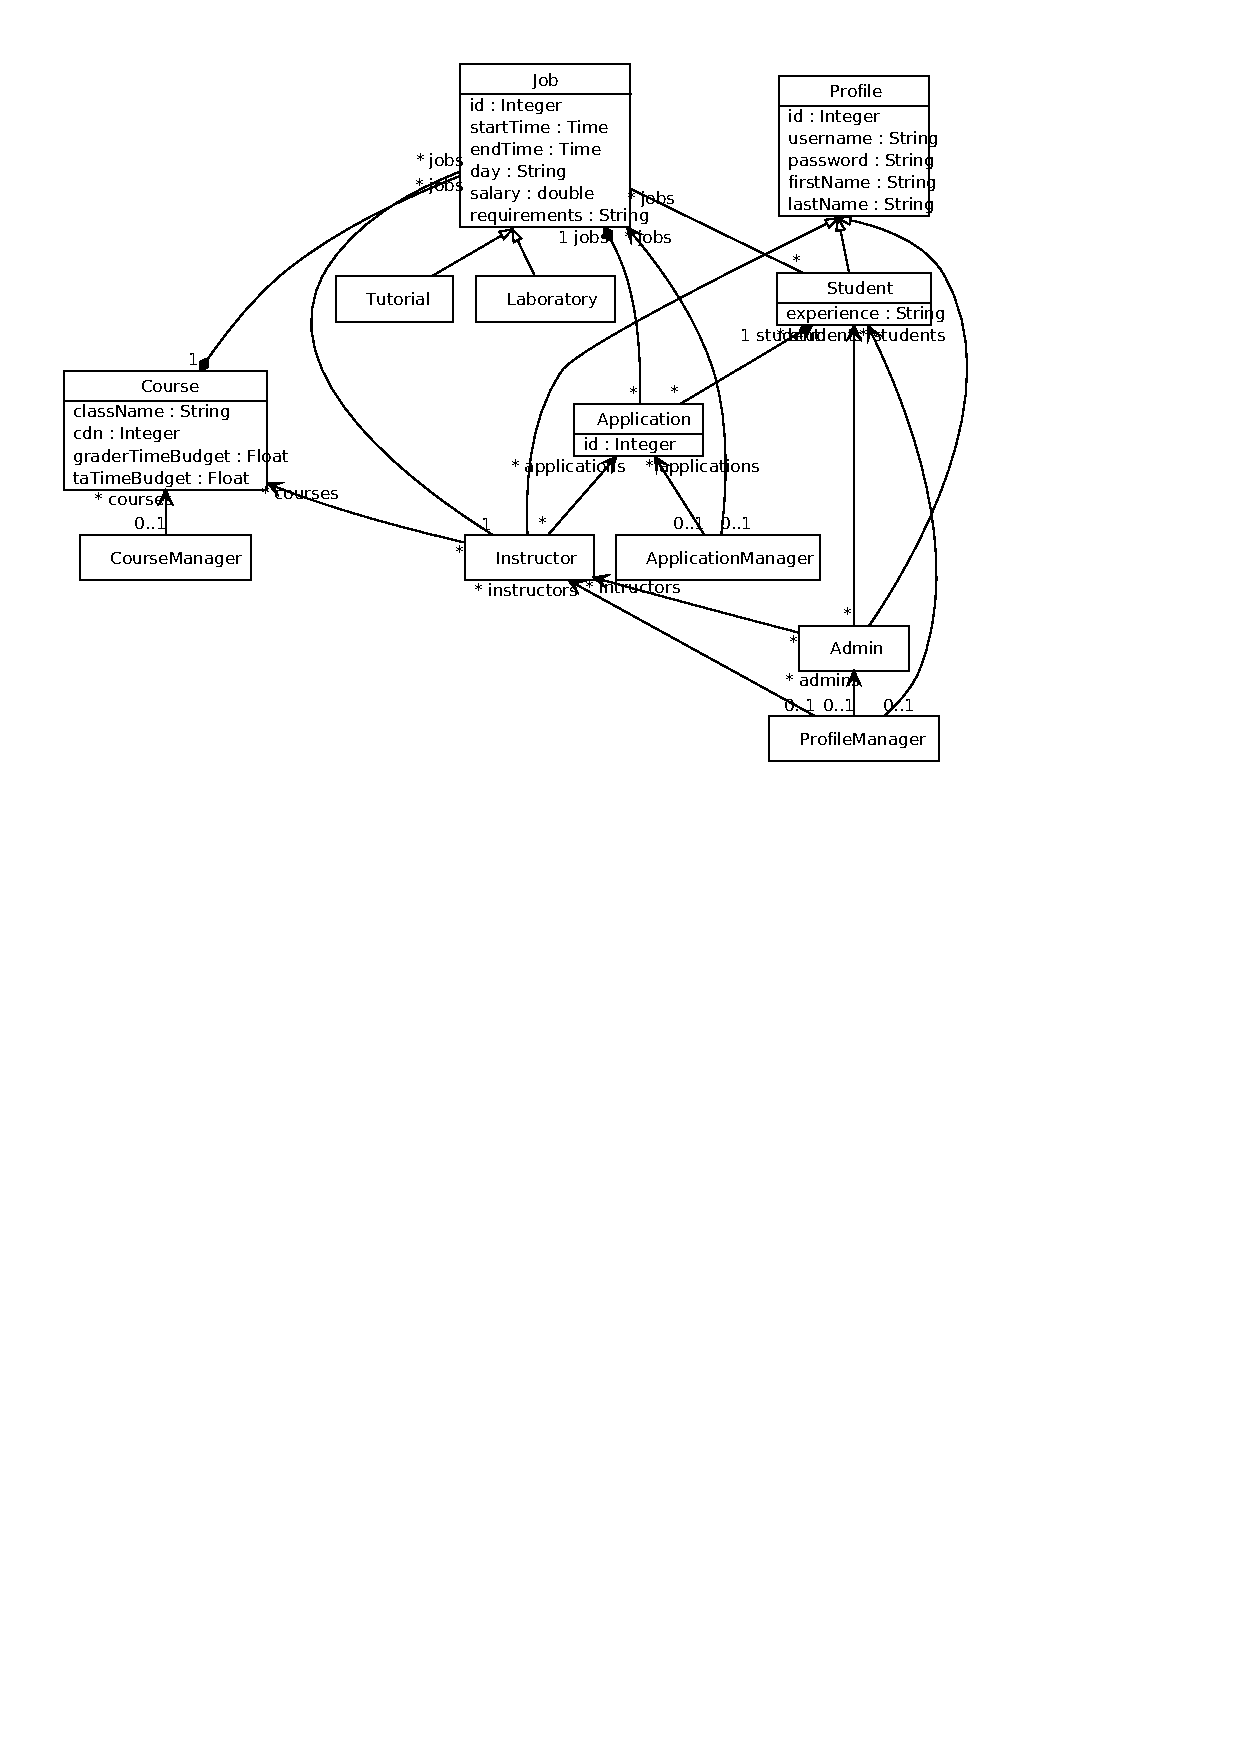
\includegraphics[scale=0.9, viewport=0 500 900 900]{model/alternateModelDiagram}
\section{Description}
\subsection{Detailed Domain Model}
The Detail Design Diagram consists of the following entities: ApplicationManager, ProfileManager,
CourseManager, Application, Profile, Course, Job, Instructor, Admin, Student, Laboratory, and
Tutorial. It consists of a Controller, called Controller, a Boundary, called View, and a
Persistence, called Persistence XStream. The Controller uses the entities ApplicationManager,
ProfileManager, and CourseManager to save, edit, and modify data within the model, which are then
saved within a persistence layer. The functionalities of the three "Manager" classes are listed
below.
\begin{itemize}
	\item The ApplicationManager is in charge of Applications, which represent the job application
		created and submitted
		by the student for a job. Furthermore, the ApplicationManager is also in charge of managing
		Job data. It is associated with Application, Job, and ProfileManager.
	\item ProfileManager creates and manages Admin, Instructor, and Student entities, all of which inherit from
		the Profile class.
	\item CourseManager creates and manages Course entities.
\end{itemize}
\subsection{Controller Classes}
In total there will be three controller classes in the Controller Packages with an additional class
for input exceptions or input validation. Each controller class has an associated Manager class, and
is in charge of utilizing the manager class safely so that appropriate data is guaranteed to be
entered into the persistence layer.\\
The Controller classes serve the purpose of isolating the model from the input, keeping in mind the
philosophies of the Model-View-Controller paradigm.
\subsection{View Classes}
Finally, there are multiple View classes, dependent on the application platform, that act as
boundary classes. These classes are in charge of gathering user input in a user-friendly manner. The
Web and Mobile applications have four and two Views, respectively, and the Desktop application has
five Views.\\
The View classes are listed by platform below:
\subsubsection{Current Desktop Views}
\begin{enumerate}
	\item \texttt{MenuView}: Allows user to select which functionality to perform
	\item \texttt{RegisterView}: Allows user to enter profile information to create a
		\texttt{Student}, \texttt{Instructor}, or \texttt{Administrator}
	\item \texttt{CreateCourseView}: Allows user to enter data to create a \texttt{Course} given a specific
		\texttt{Instructor}
	\item \texttt{PublishJobView}: Allows user to enter information required for creating a
		\texttt{Job}
	\item \texttt{ApplicationView}: Allows user to create an \texttt{Application}
\end{enumerate}
\subsubsection{Current Mobile Views}
\begin{enumerate}
	\item \texttt{MainActivity}: Allows user to select which functionality to perform (analogous to
		\texttt{MenuView})
	\item \texttt{ApplyToJob}: Allows user to create an \texttt{Application} (analogous to
		\texttt{ApplicationView})
\end{enumerate}
\subsubsection{Current Web Views}
\begin{enumerate}
	\item \texttt{index}: Allows user to select which functionality to perform (analogous to
		\texttt{MenuView})
	\item \texttt{createCourse}: Allows user to enter data to create a \texttt{Course} (analogous to
		\texttt{CreateCourseView})
	\item \texttt{createInstructor}: Allows user to enter data to create an \texttt{Instructor}
		(analogous to \texttt{RegisterView}). This View is temporary and will only be used for this
		Deliverable, as it does not satisfy the requirements of the project.
	\item \texttt{job}: Allows user to submit data to publish a \texttt{Job} (analogous to
		\texttt{PublishJobView})
\end{enumerate}
\section{Rationale}
The program was designed this way so as to follow the principles of the Model-View-Controller design
pattern. As discussed previously, this allowed for the effective isolation of the user input and the
domain model. The Controller classes, along with the \texttt{PersistenceXStream} class, allow for
persistence to be carried out in a safe manner. The Controller classes are designed in such a way
that by using them to create their associated objects, the created objects will automatically be
stored within the persistence layer assuming they were created successfully. To avoid storing faulty
objects, the \texttt{InputException}, as well as several validation classes in PHP, were created. As
such, the Controller classes throw exceptions when unworthy data is passed. The ultimate benefit to
using this design is that the persistence is taken care of at the level of the controller classes,
so the programmer needn't worry about it when designing the Views. With this foundation, the model
may be altered reliably.\\\\
By perusing the list of Views, it is clear that the mobile and web Views are very similar to the
desktop Views in terms of their purposes. This was done to create consistent interfaces across the
platforms. The desktop has many views because it is meant to be used by Administrators, who can
implement the functionalities possible on all other platforms.
\section{Detailed Design Diagram}
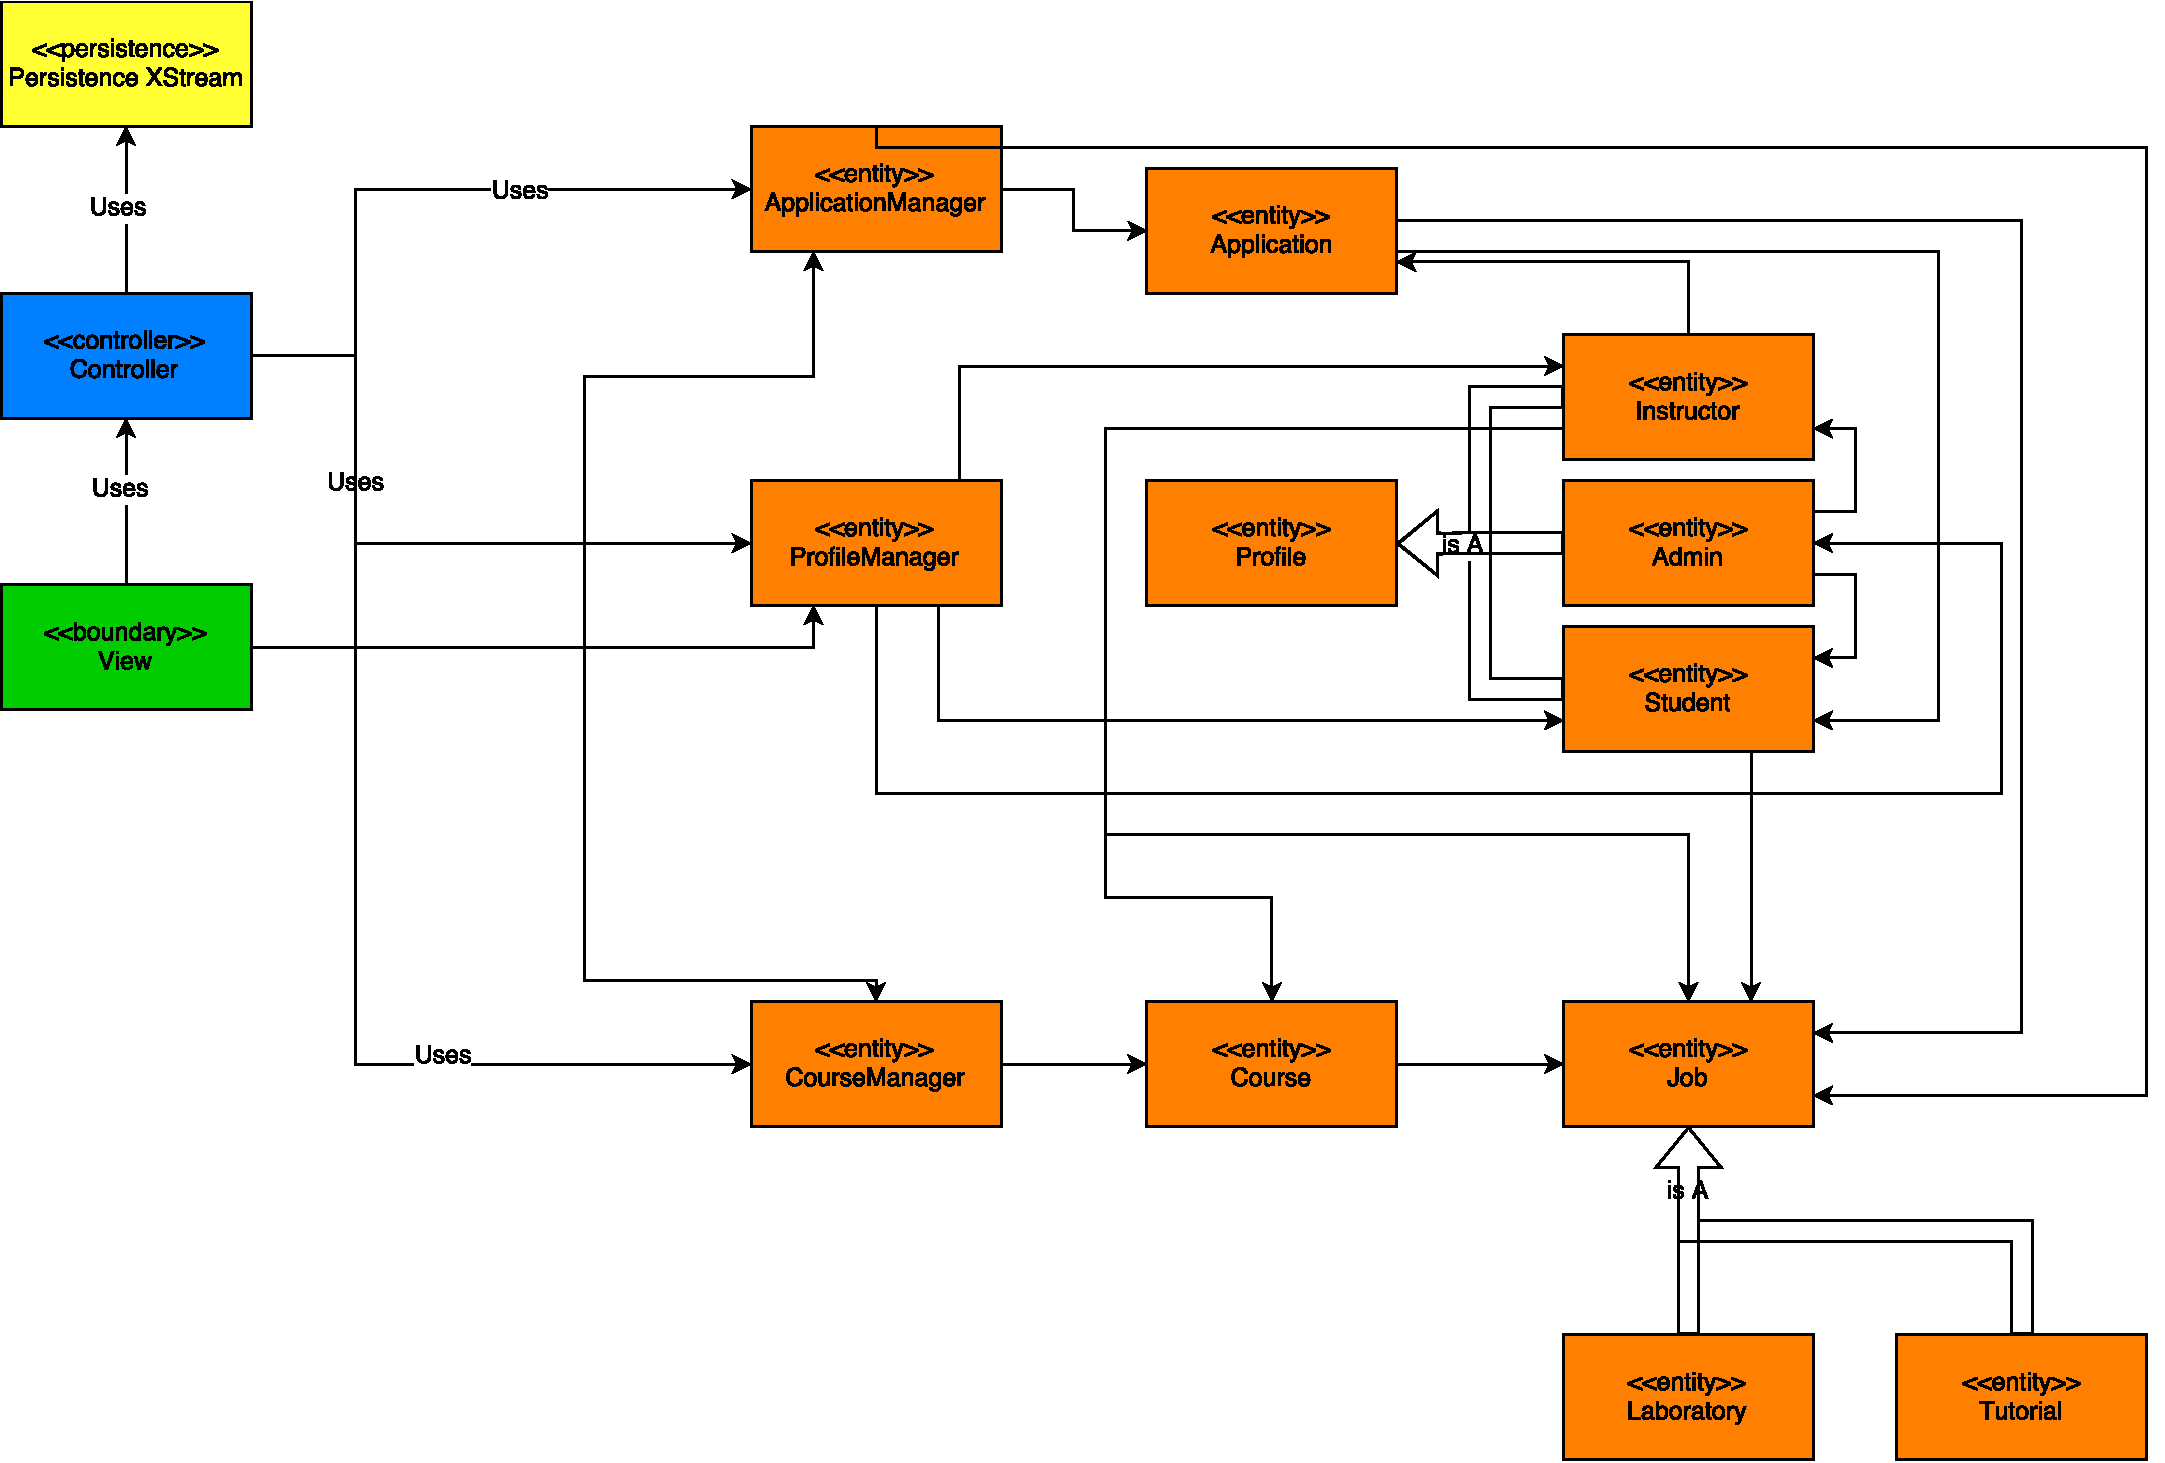
\includegraphics[scale=0.6,angle=270]{DetailedDomainModelDiagram}
\section{Java and Android Controller Class Diagram (Desktop and Mobile)}
\begin{figure}[H]
	\centering
	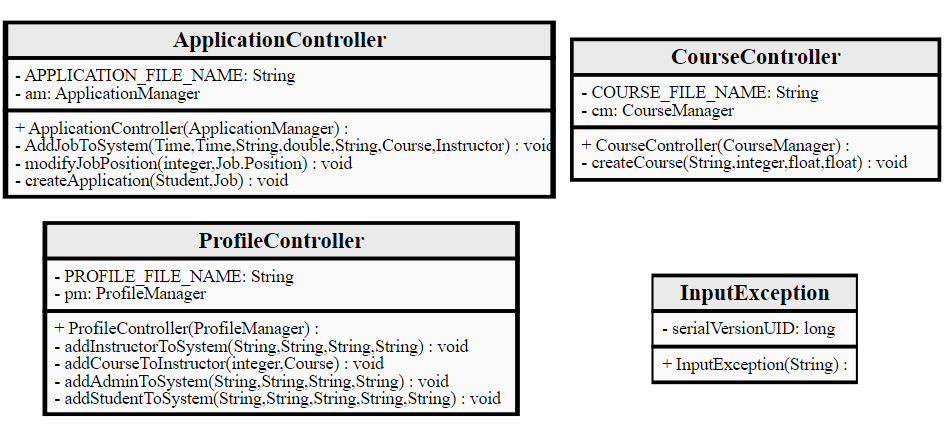
\includegraphics[scale=0.95]{./Design/ClassDiagrams/ControllerPackageClassDiagramJava}
\end{figure}
\section{PHP Controller Class Diagram (Web)}
\begin{figure}[H]
	\centering
	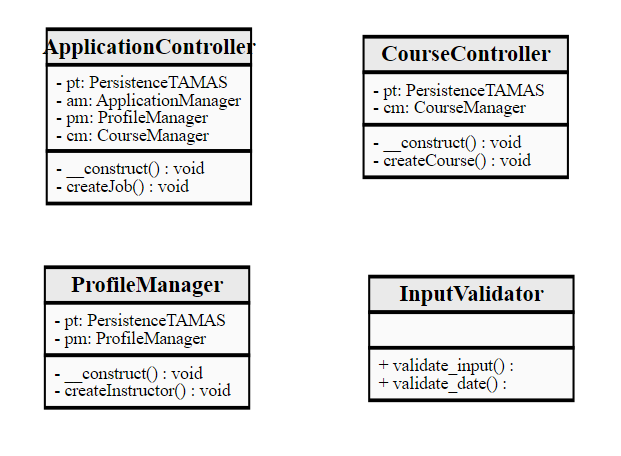
\includegraphics[scale=1.05]{./Design/ClassDiagrams/ControllerPackageClassDiagramPHP}
\end{figure}
\section{Java View Class Diagram (Desktop)}
\begin{figure}[H]
	\centering
	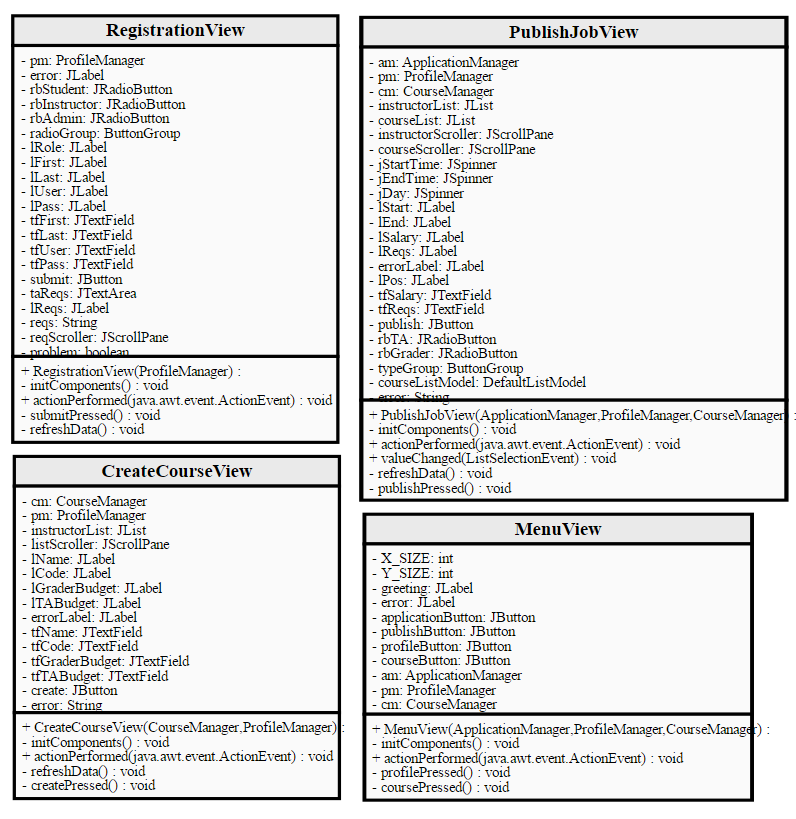
\includegraphics[scale=1]{./Design/ClassDiagrams/desktopViewPackageDiagram(A)}
	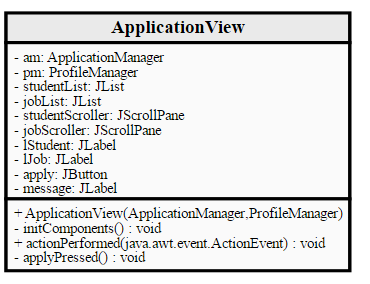
\includegraphics[scale=1]{./Design/ClassDiagrams/desktopViewPackageDiagram(B)}
\end{figure}
\section{PHP View Class Diagram (Web)}
\begin{figure}[H]
	\centering
	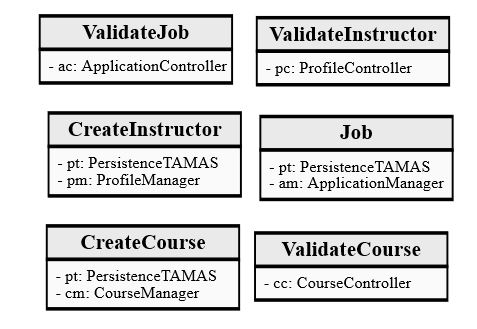
\includegraphics[]{./Design/ClassDiagrams/WebViewPackageDiagram}
\end{figure}
\section{Android View Class Diagram (Android)}
\begin{figure}[H]
	\centering
	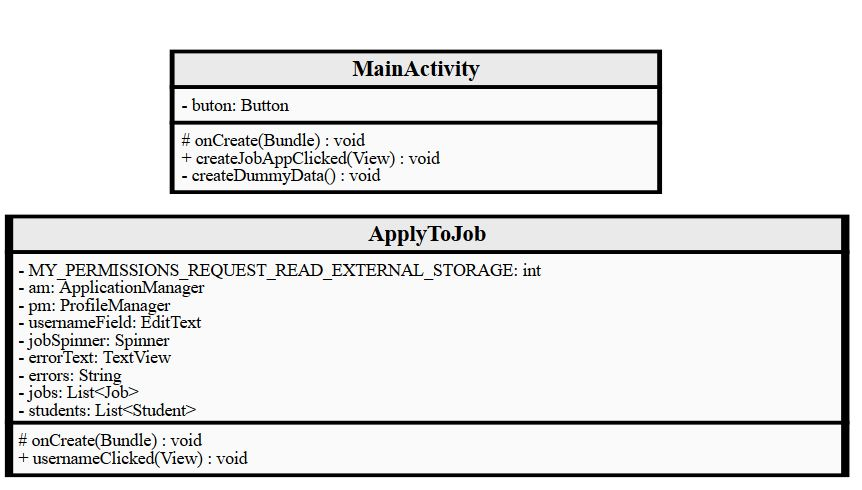
\includegraphics[]{./Design/ClassDiagrams/AndroidViewPackageDiagram}
\end{figure}

\part{Implementation of Prototypes}

\section{Desktop Application}
The desktop application submitted in this Deliverable contains all functionalities necessary to
generate the sufficient entities to complete the following required use cases: Apply to Job
(Desktop), Apply to Job (Mobile), Publish Job Posting (Desktop). This includes the abilities to
create profiles, create courses, create job postings, and submit job applications. All of the
mentioned functionalities are persisted, so the XML files that are output may be used as data for
the other platforms. Below are the sequence diagrams describing the desktop use cases.
\subsection{Desktop Publish Job Posting Use Case}
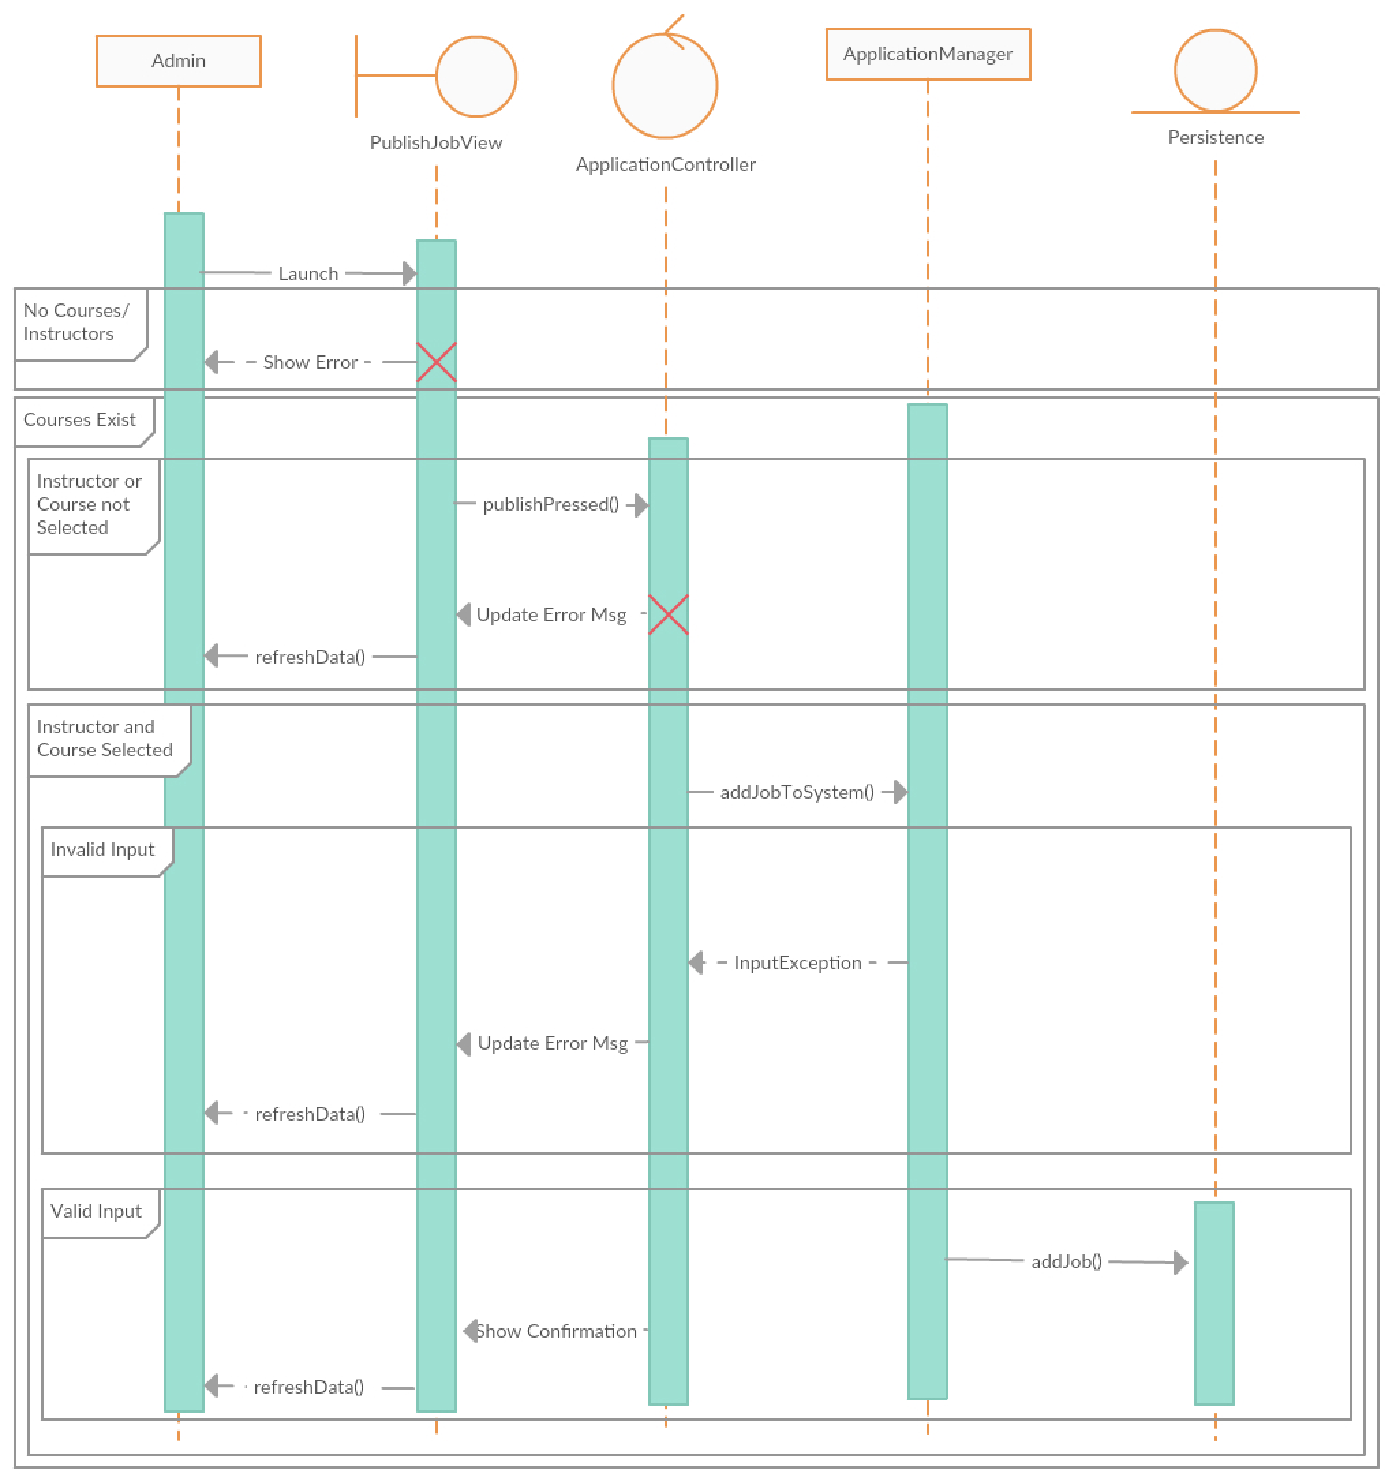
\includegraphics[scale=0.73]{model/SEQUENCE/publish_desktopSequenceAlt}
\subsection{Desktop Apply to Job Use Case}
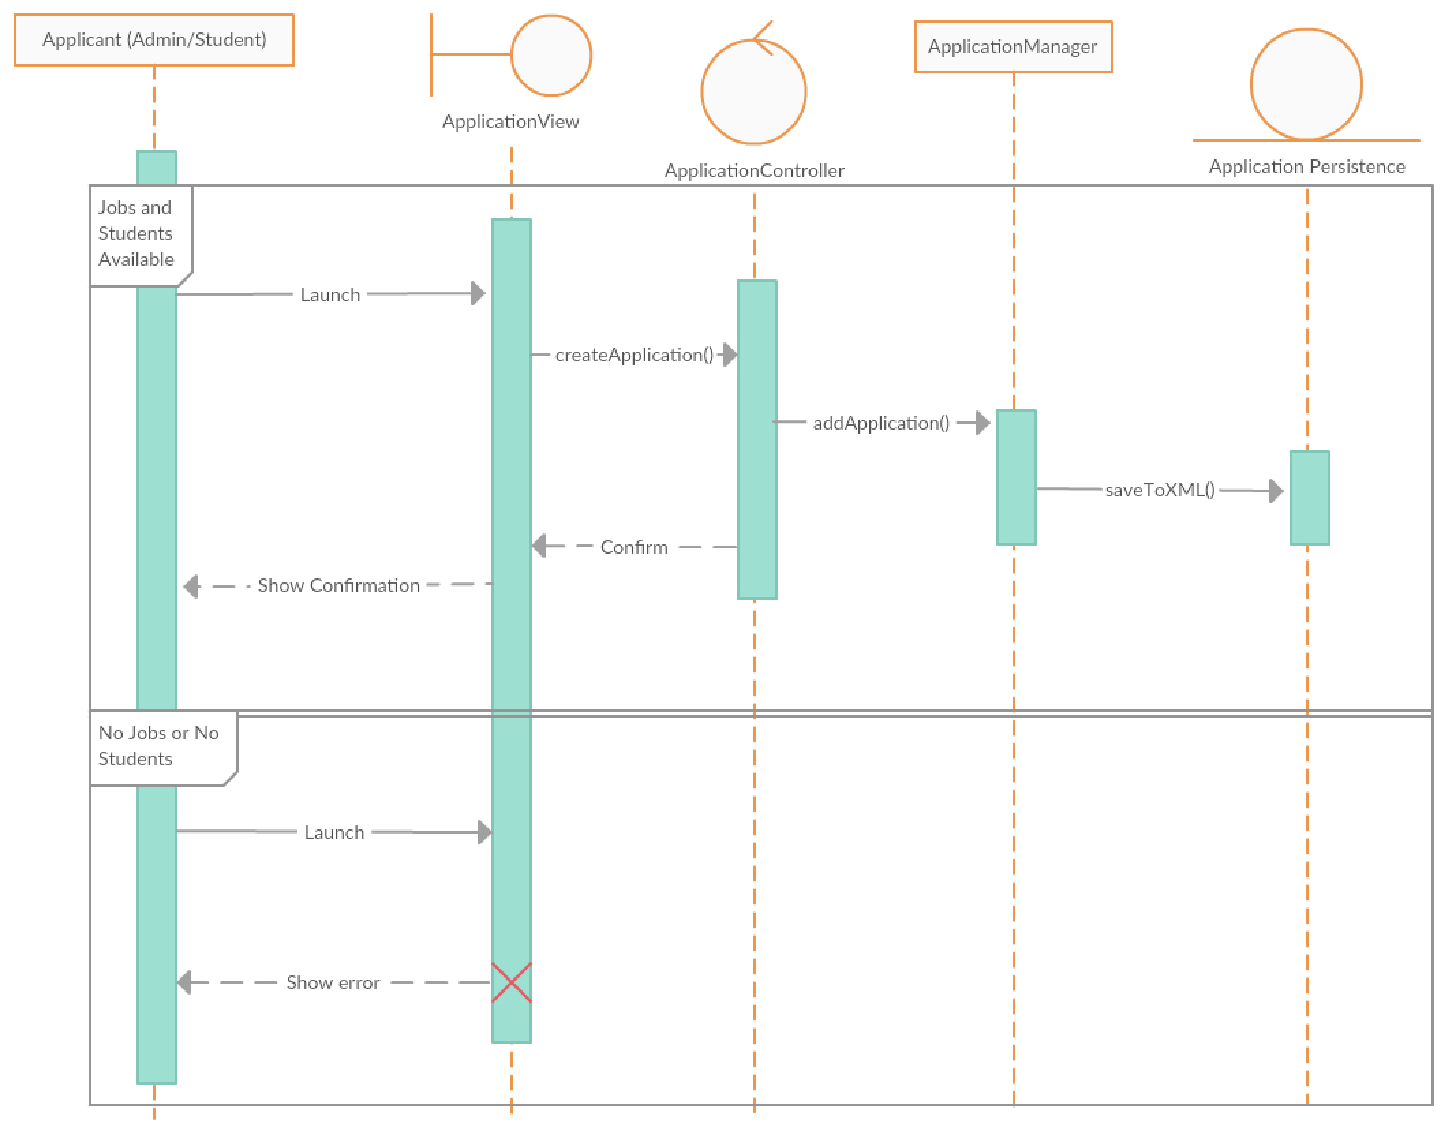
\includegraphics[scale=0.73]{model/SEQUENCE/apply_desktopSequence}

\section{Web Application}
The web application submitted in this Deliverable contains all functionalities required to complete
the required Publish Job Posting (Web) use case. This means that the web application must be capable
of creating instructors and creating courses, otherwise the Publish Job use case could not function
without prior XML data. Although the desktop application can provide this XML data, it was easier in
the development phase if the web application could do this independently. Therefore, the ability to
create instructors and create courses is only temporary. Importantly, in publishing a job posting,
the job data is saved in the persistence layer and may copied to the appropriate directories on the
other platforms for use. Following is the sequence diagram describing the required web use case.
\subsection{Web Publish Job Posting Use Case}
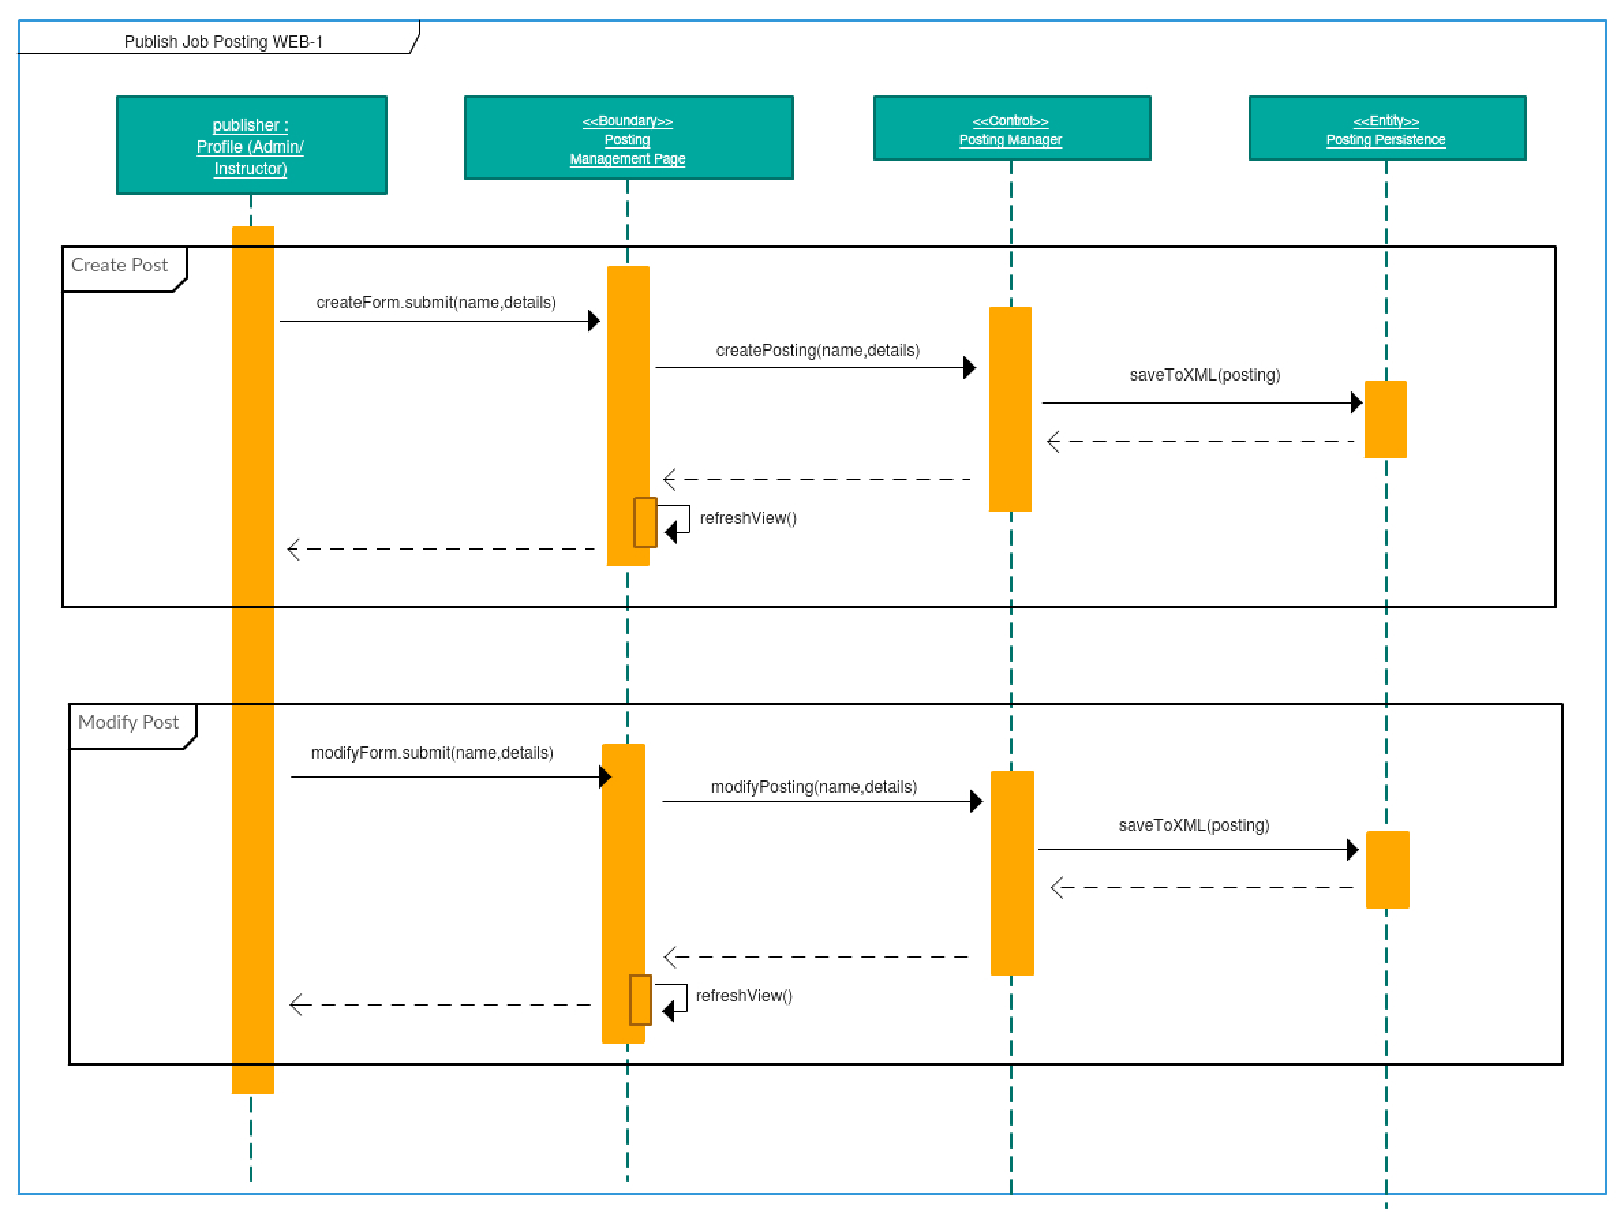
\includegraphics[scale=0.73]{model/SEQUENCE/publish_webSEQUENCE1}\\
Continued on next page\dots\newpage
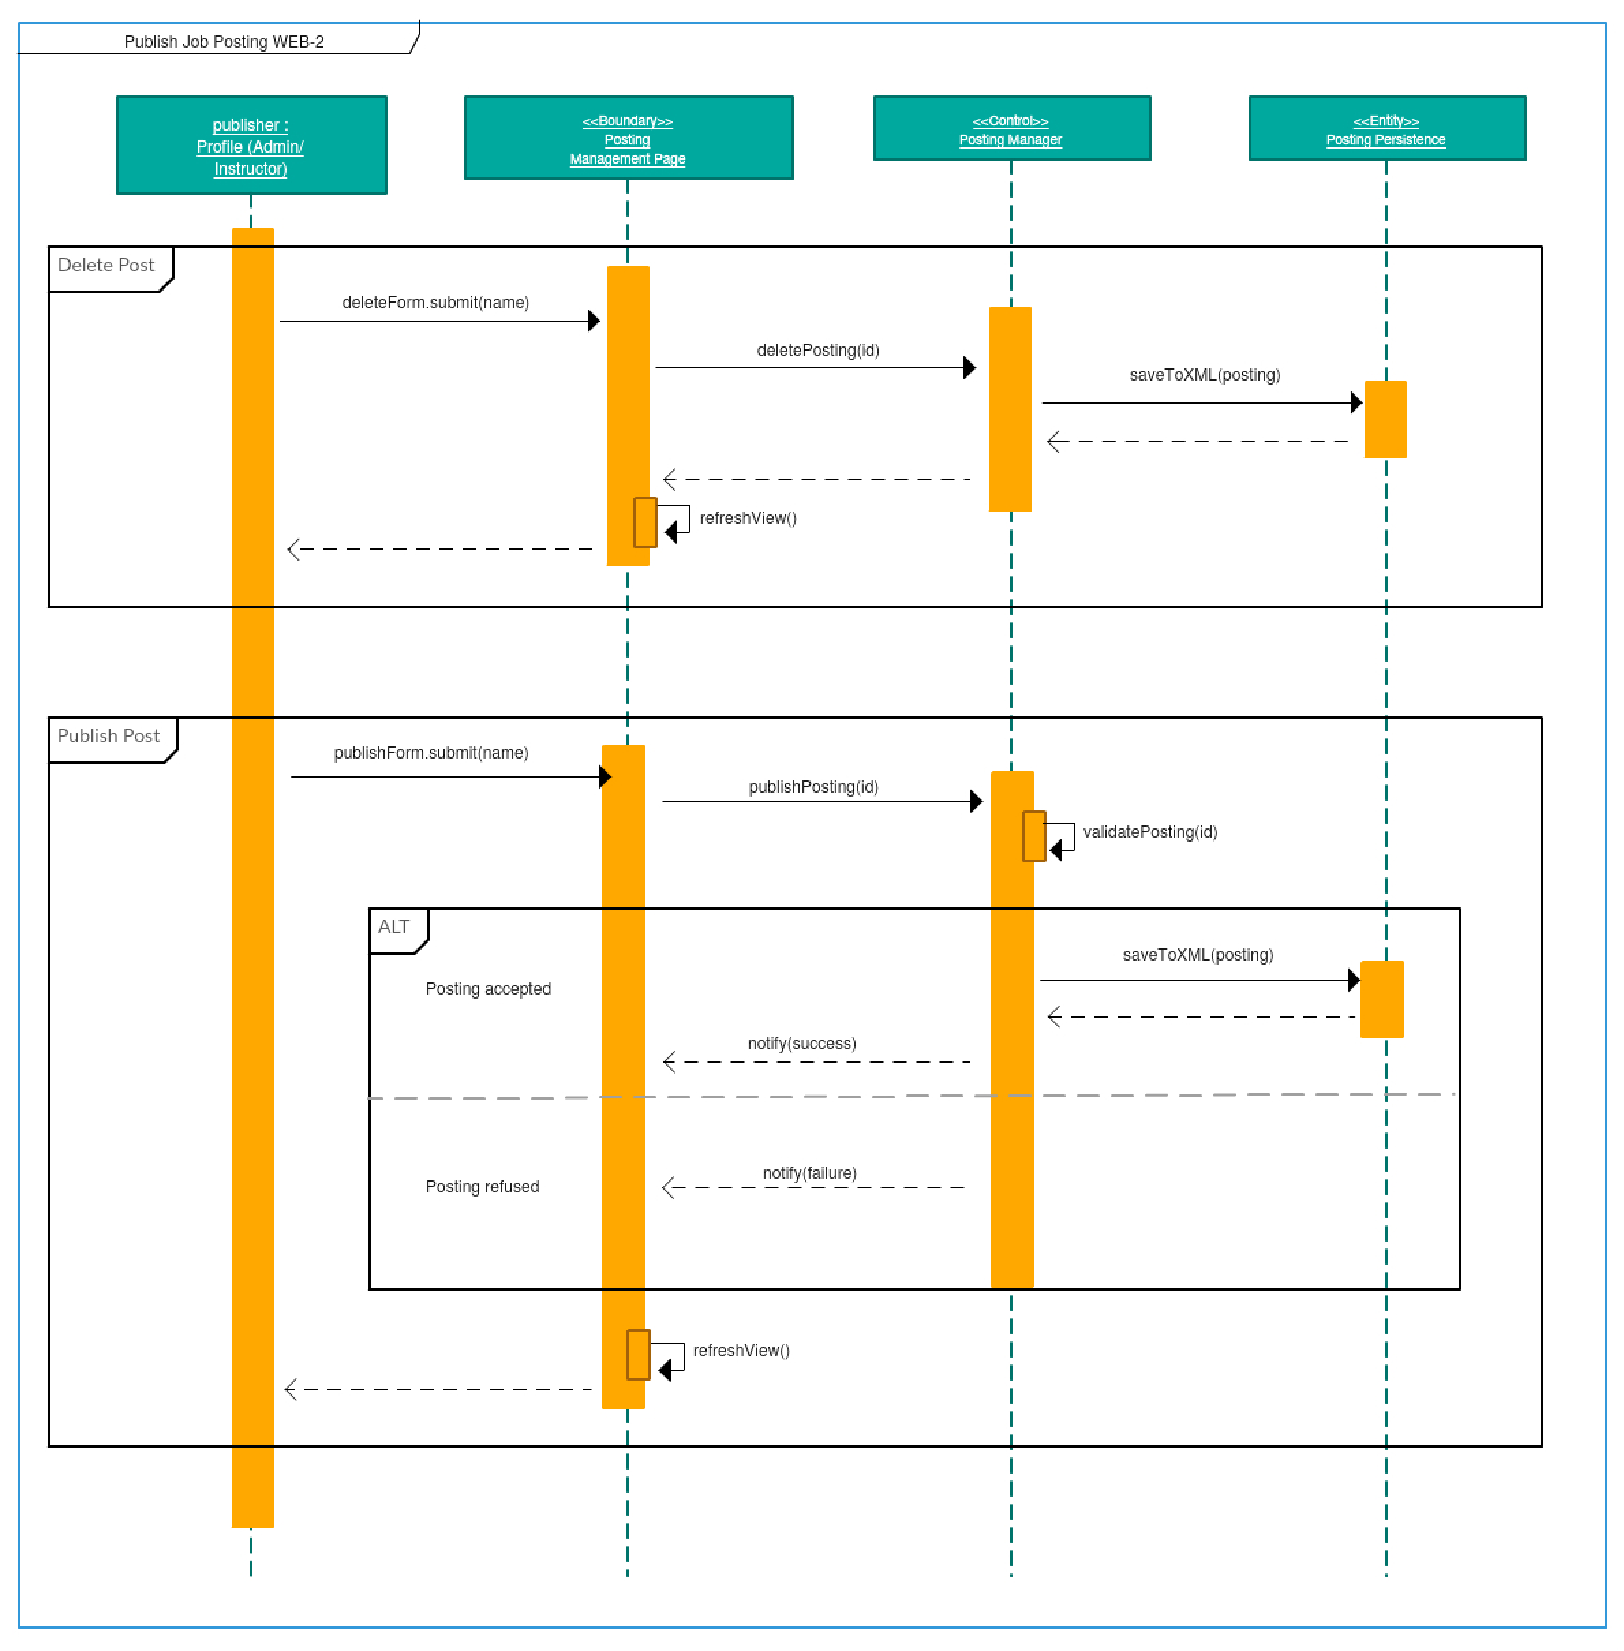
\includegraphics[scale=0.73]{model/SEQUENCE/publish_webSEQUENCE2}

\section{Mobile Application}
The mobile application submitted in this Deliverable has the ability to complete the Apply to Job
Posting (Mobile) use case, given prior XML data. For convenience, the mobile application generates
sample entities if it is found that there is no data, to make testing and validation easier.
However, should someone wish to use their own XML data to test the application, this is possible by
placing the XML files (say, that were generated from the desktop application) in the following
directory: \texttt{/storage/emulated/0/Android/obb/ca.mcgill.ecse321.group10.tamas/}. This, of
course, is also the directory of the output persistence of the mobile app. In applying to a job, the
mobile application saves the \texttt{Application} data to a persistence XML file which can then be
used on the other platforms. Below is the sequence diagram representing the required mobile use
case.
\subsection{Mobile Apply to Job Posting Sequence Diagram}
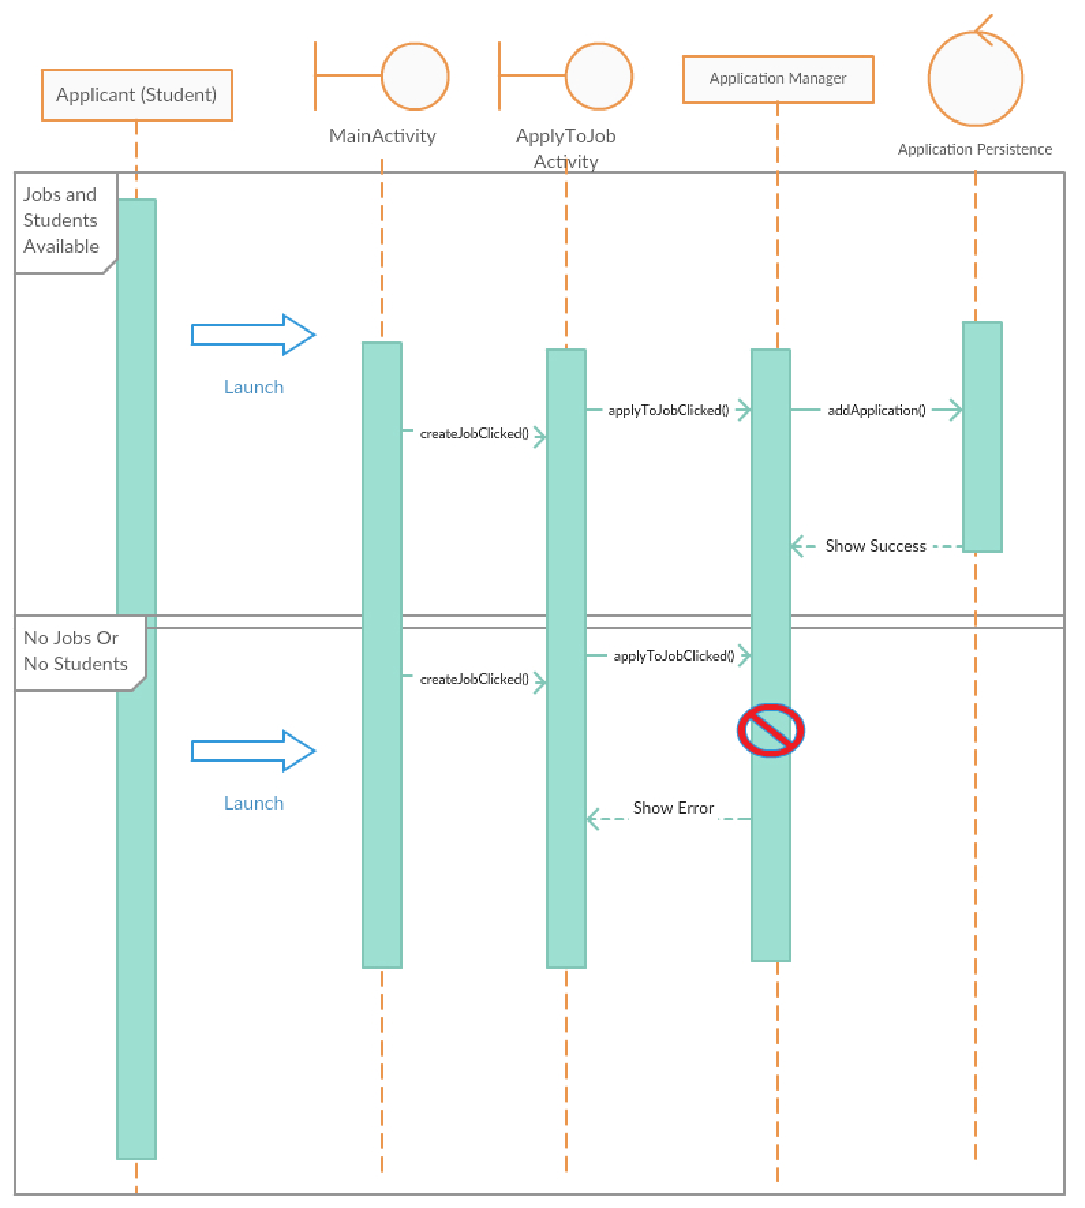
\includegraphics[scale=0.90]{model/SEQUENCE/apply_mobileSEQUENCE}

\part{Work Plan From Past and Future Iterations}
In this section, the updated workplan may be pondered. The full detailed backlog including work
hours per team member, key decisions, and work history may be seen on the remote git repository's
root directory in the file called \texttt{backlog.pdf}.
\subsection{Iteration 1}

In the following week, we will create more detailed sequence diagrams going into the details of the
implementations on individual platforms. We will then develop prototype source code for the Publish
Job Posting and Apply for Job use cases for the desktop and mobile applications respectively.

\subsection{Iteration 2}

In the following Deliverable, thorough testing needs to be completed. The following are deadlines
and the estimated effort it will take to complete these tasks on a scale of 1 to 10.

\begin{itemize}
	\item March 10 - First iteration of unit tests for Apply to Job and Publish Job posting on web,
		desktop and mobile. Estimated Effort: 8/10
	\item March 13 - Second iteration of unit tests for Apply to Job and Publish Job posting on web,
		desktop and mobile. Estimated Effort: 6/10
	\item March 13 - First iteration of System and Component tests. Estimated Effort: 6/10
    \item March 15 - First iteration of Stress Testing and Final iteration of unit tests. Estimated Effort: 6/10
    \item March 16 - First iteration of Descriptions of all tests done. Estimated Effort: 5/10
	\item March 10 - Deadline for Deliverable 3, including editing of backlog and update of
		workplan. Estimated Effort: 4/10

\end{itemize}

%\subsection{Detailed Domain Model}
%The three Manager classes were needed in order to give functionality to the user to create the
%entities associated with the manager classes, except for ApplicationManager creating a
%ProfileManager. The reason ApplicationManager is associated to ProfileManager is because otherwise
%the only way for ApplicationManager to have access to Student is by a direct association to it; this
%would cause a redundancy as now two manager classes are able to create Student entities, which is
%something we want to avoid. Having a separate controller for each manager class allows one to modify
%the functionality of one controller class with its respective manager class without it having to
%affect the other controller classes.
\end{document}
